	\newpage
\section{Podręcznik użytkownika}  %6
%Opis jak używać programu. Mogą być z zrzut ekranu razem z opisem. 

Przed włączeniem aplikacji należy upewnić się, że w telefonie użytkownika zapisany jest odcisk palca. Jest on potrzebny do dostania się do aplikacji. 

\begin{figure}[H]
	\centering
	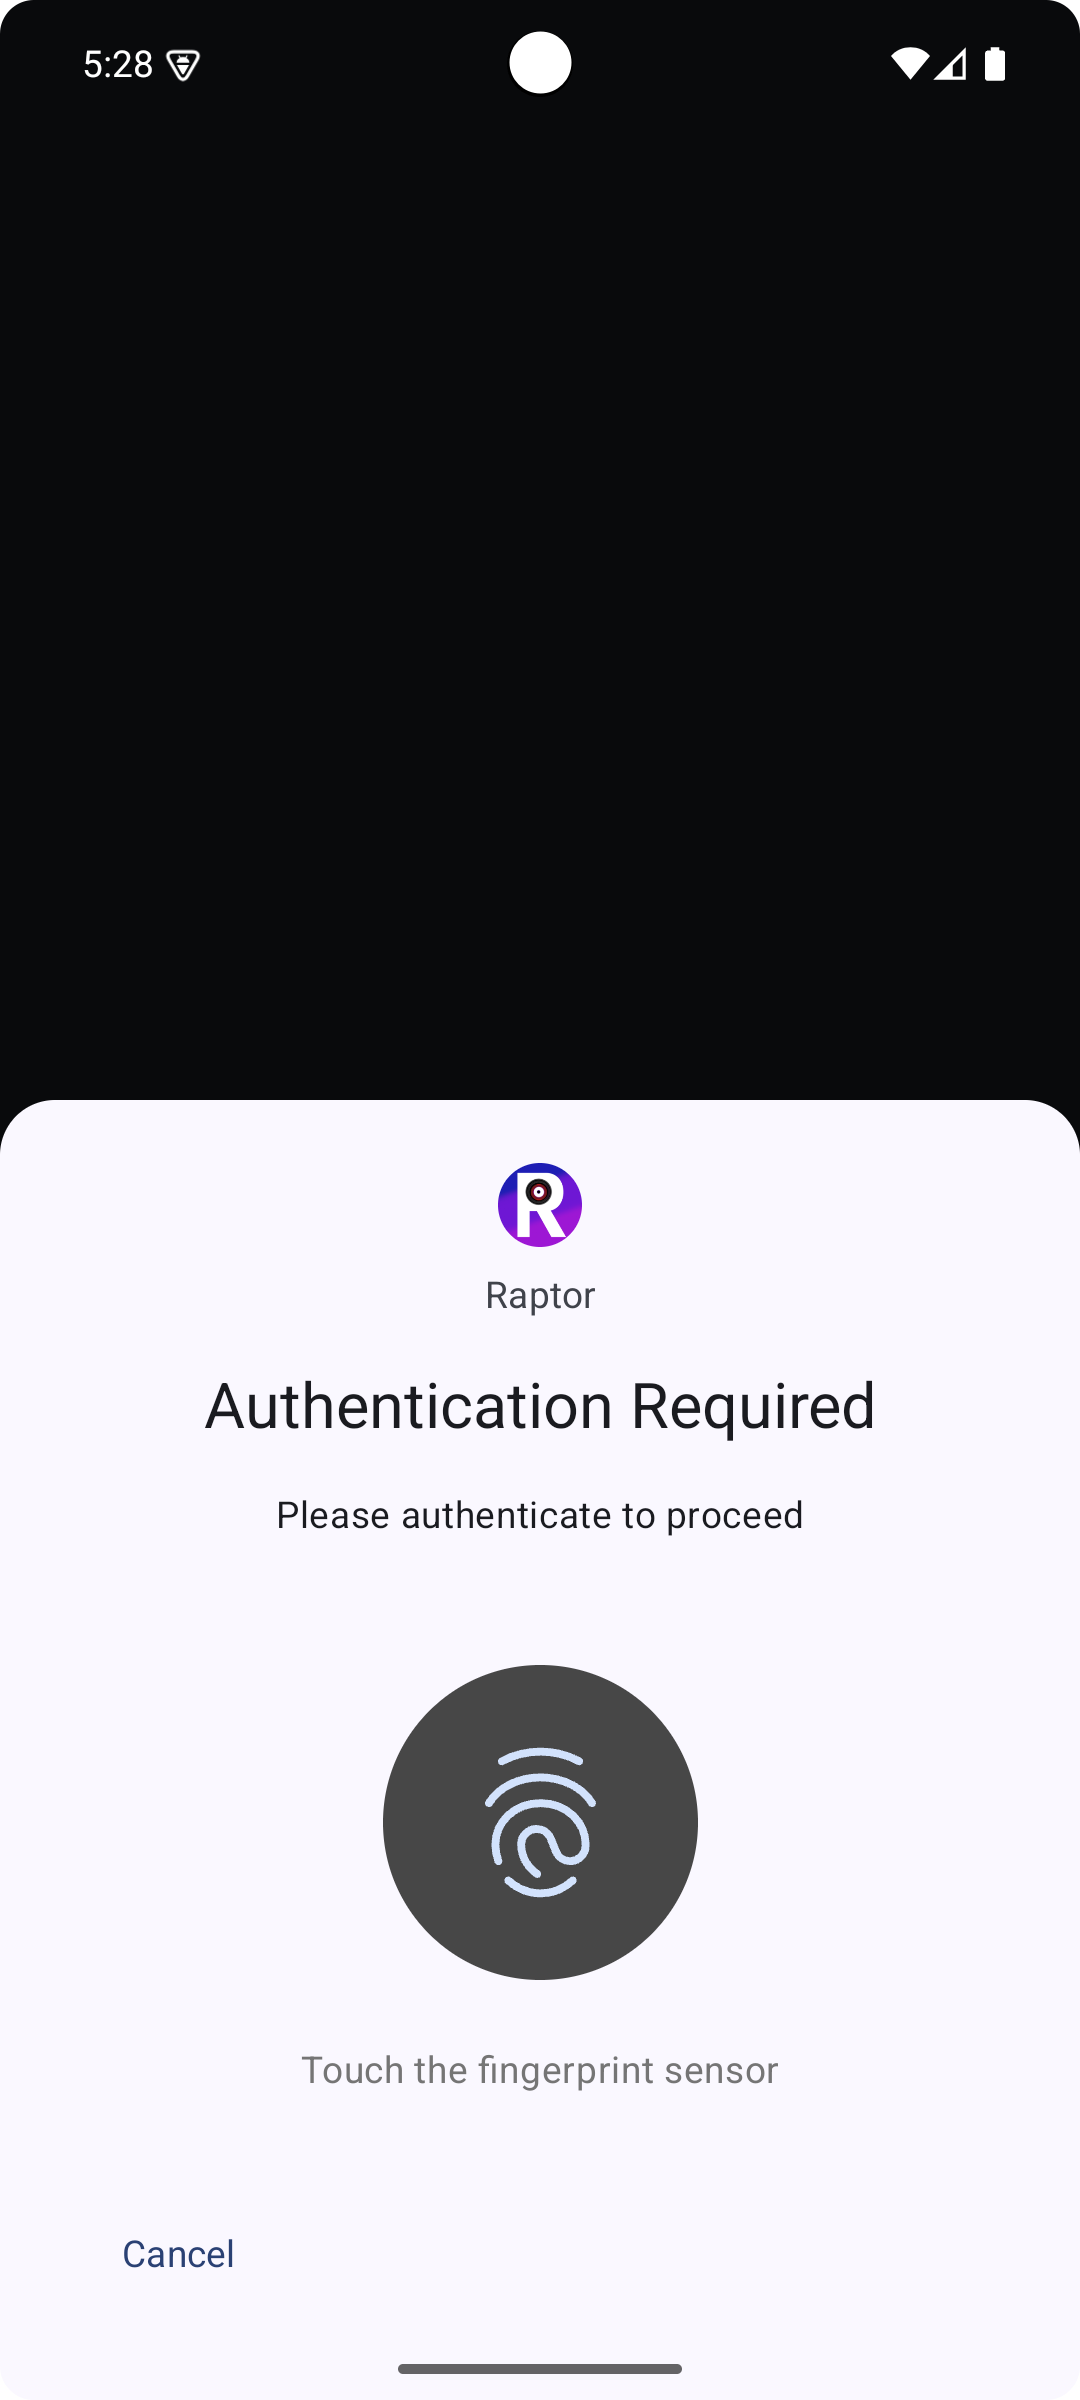
\includegraphics[width=1\textwidth]{images/usage_fingerprint.png}
	\caption{\centering{Prośba o podanie odcisku palca.}}
	\label{fig:usage_fingerprint}
\end{figure}

Po włączeniu aplikacji użytkownik zostanie poproszony o podanie odcisku palca jak widać na rysunku nr.~\ref{fig:usage_fingerprint}. Po zweryfikowaniu, aplikacja przechodzi na główny ekran. Domyślnie, wygląda on jak na rysunku nr.~\ref{fig:tutorial_autorzy_pusty}

\begin{figure}[H]
	\centering
	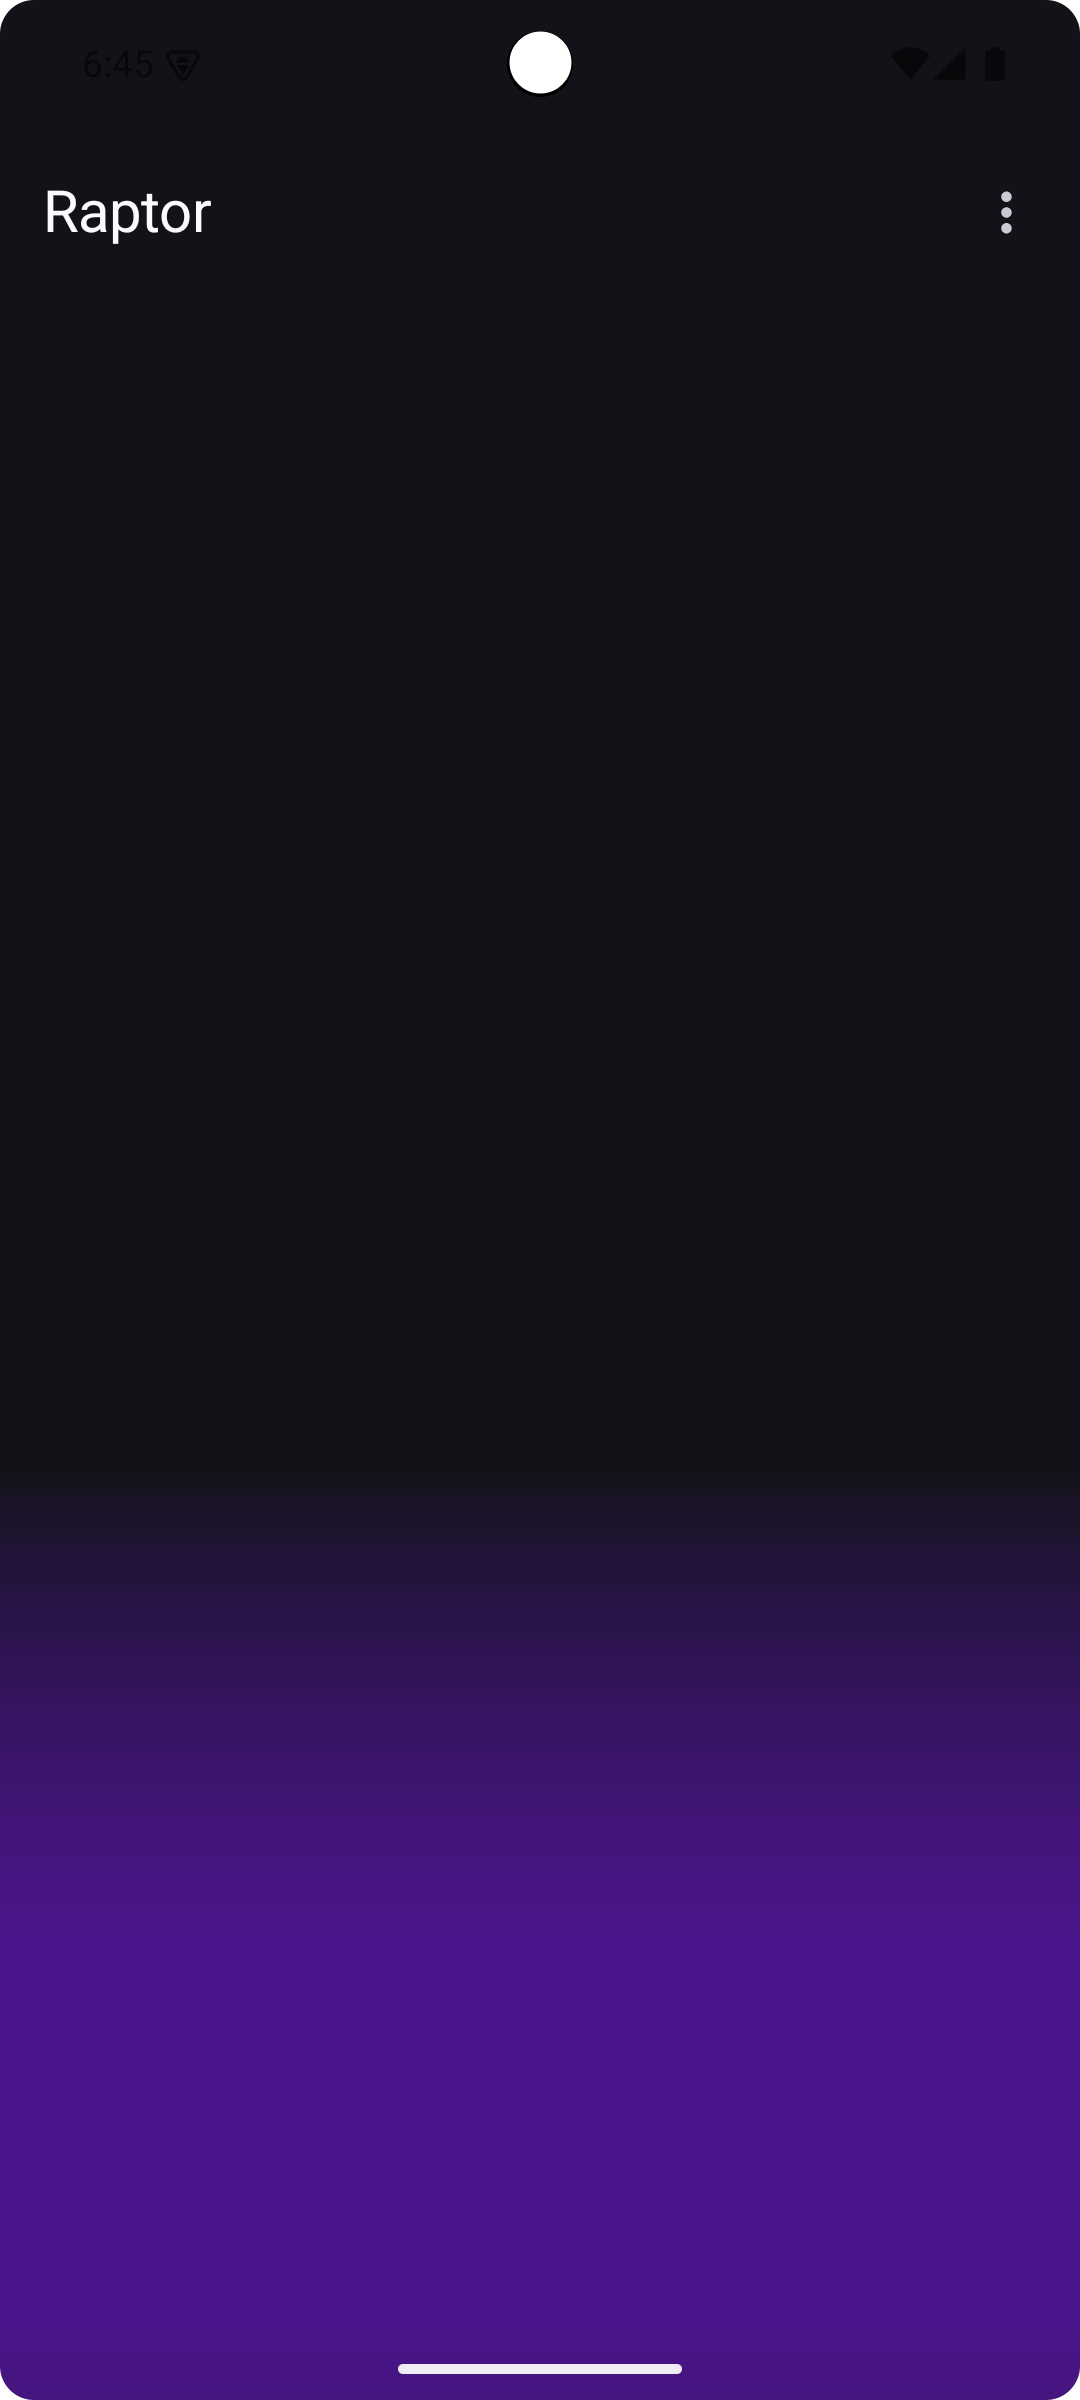
\includegraphics[width=1\textwidth]{images/tutorial_autorzy_pusty.png}
	\caption{\centering{Widok po zweryfikowaniu odcisku.}}
	\label{fig:tutorial_autorzy_pusty}
\end{figure}

Jeżeli użytkownik chce dodać swoje piosenki, powinien nacisnąć przycisk w postaci trzech kropek w prawym górnym rogu i wybrać opcję select folder, jak widać na rysunku nr.~\ref{fig:tutorial_select_folder}.

\begin{figure}[H]
	\centering
	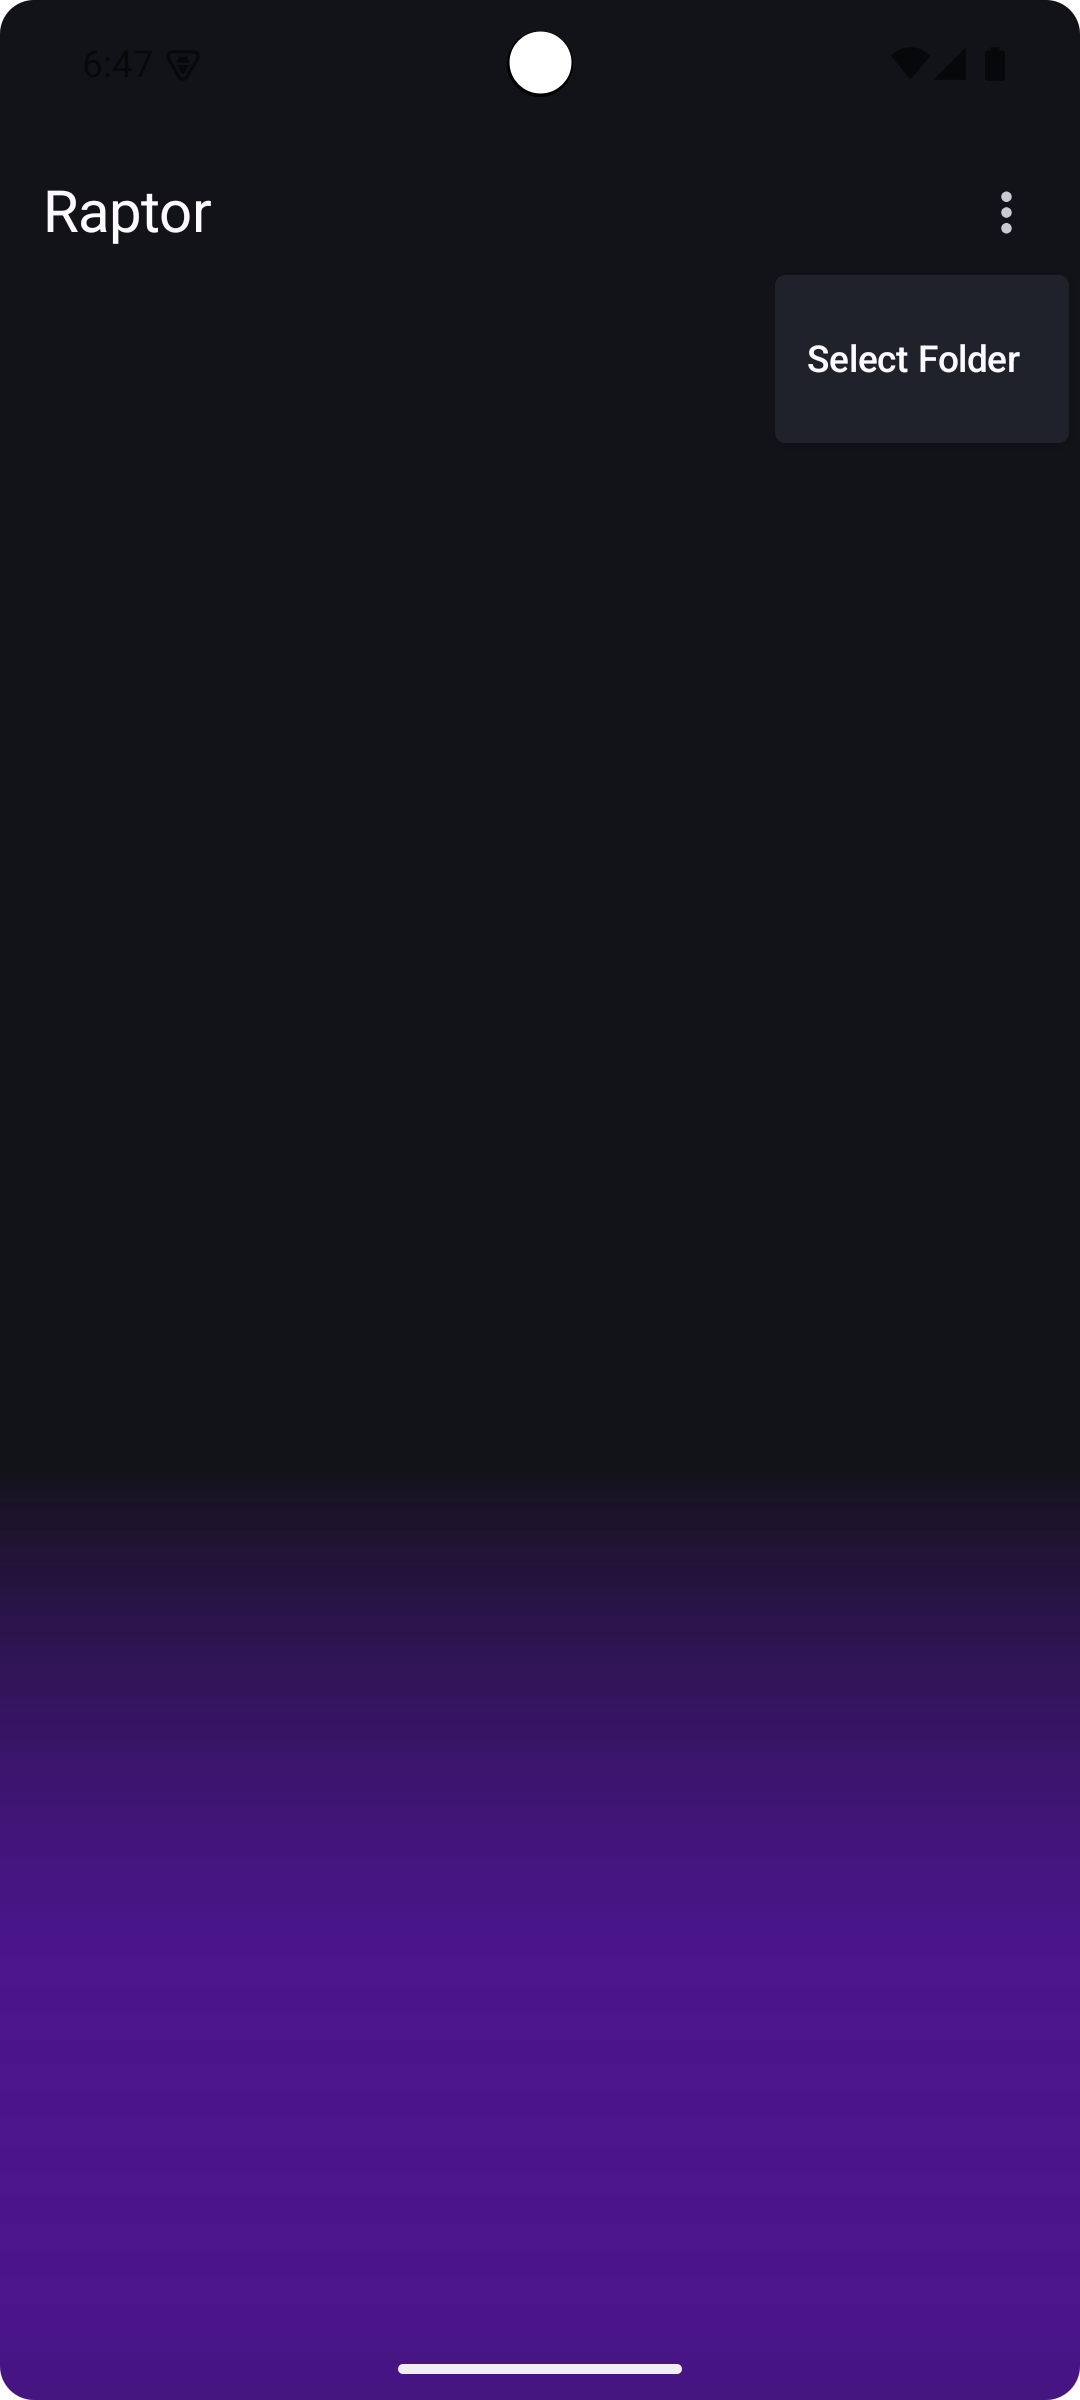
\includegraphics[width=1\textwidth]{images/tutorial_select_folder.png}
	\caption{\centering{Włączenie wyboru folderu.}}
	\label{fig:tutorial_select_folder}
\end{figure}

Otworzy się następnie systemowy dialog wyboru folderu. Użytkownik powinien wybrać jakiś, jak na rys. nr.~\ref{fig:tutorial_folder_selected}. Nie musi mieć on bezpośrednio w sobie plików z muzyką, może zawierać podfoldery.

\begin{figure}[H]
	\centering
	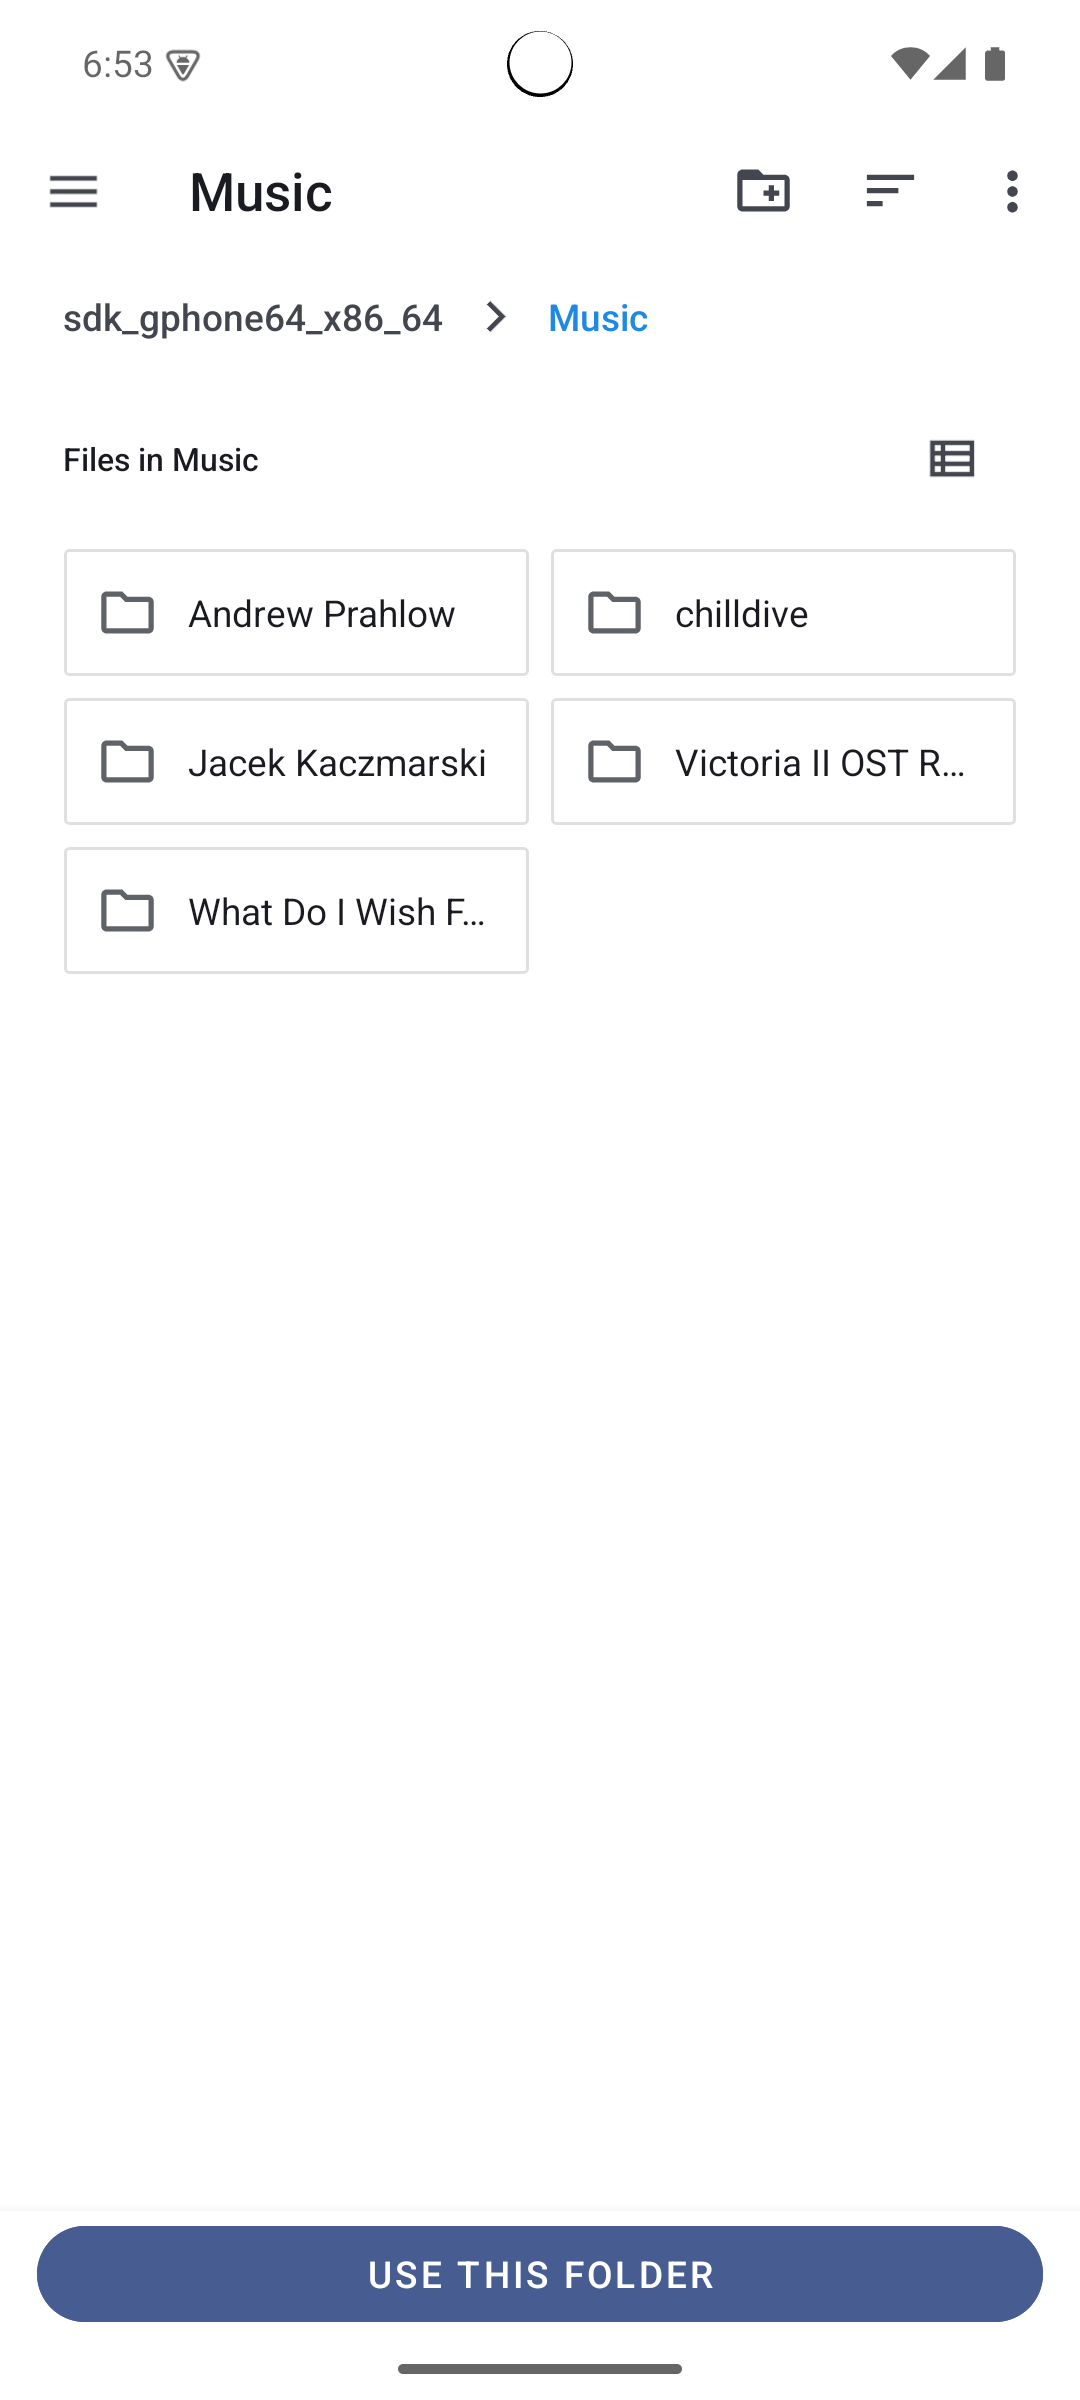
\includegraphics[width=1\textwidth]{images/tutorial_folder_selected.png}
	\caption{\centering{Wybieranie folderu z muzyką.}}
	\label{fig:tutorial_folder_selected}
\end{figure}

Po wybraniu folderu, aplikacja wraca użytkownika do ekranu głównego. Po poczekaniu chwili, pokaże się lista autorów, jakie aplikacja wykryła. Jeżeli jakieś pliki nie mają w swoich tagach autora, zostają one przypisane do sekcji \texttt{Unknown}. Nowy widok jest przedstawiony na rysunku nr.~\ref{fig:tutorial_after_loading}.

\begin{figure}[H]
	\centering
	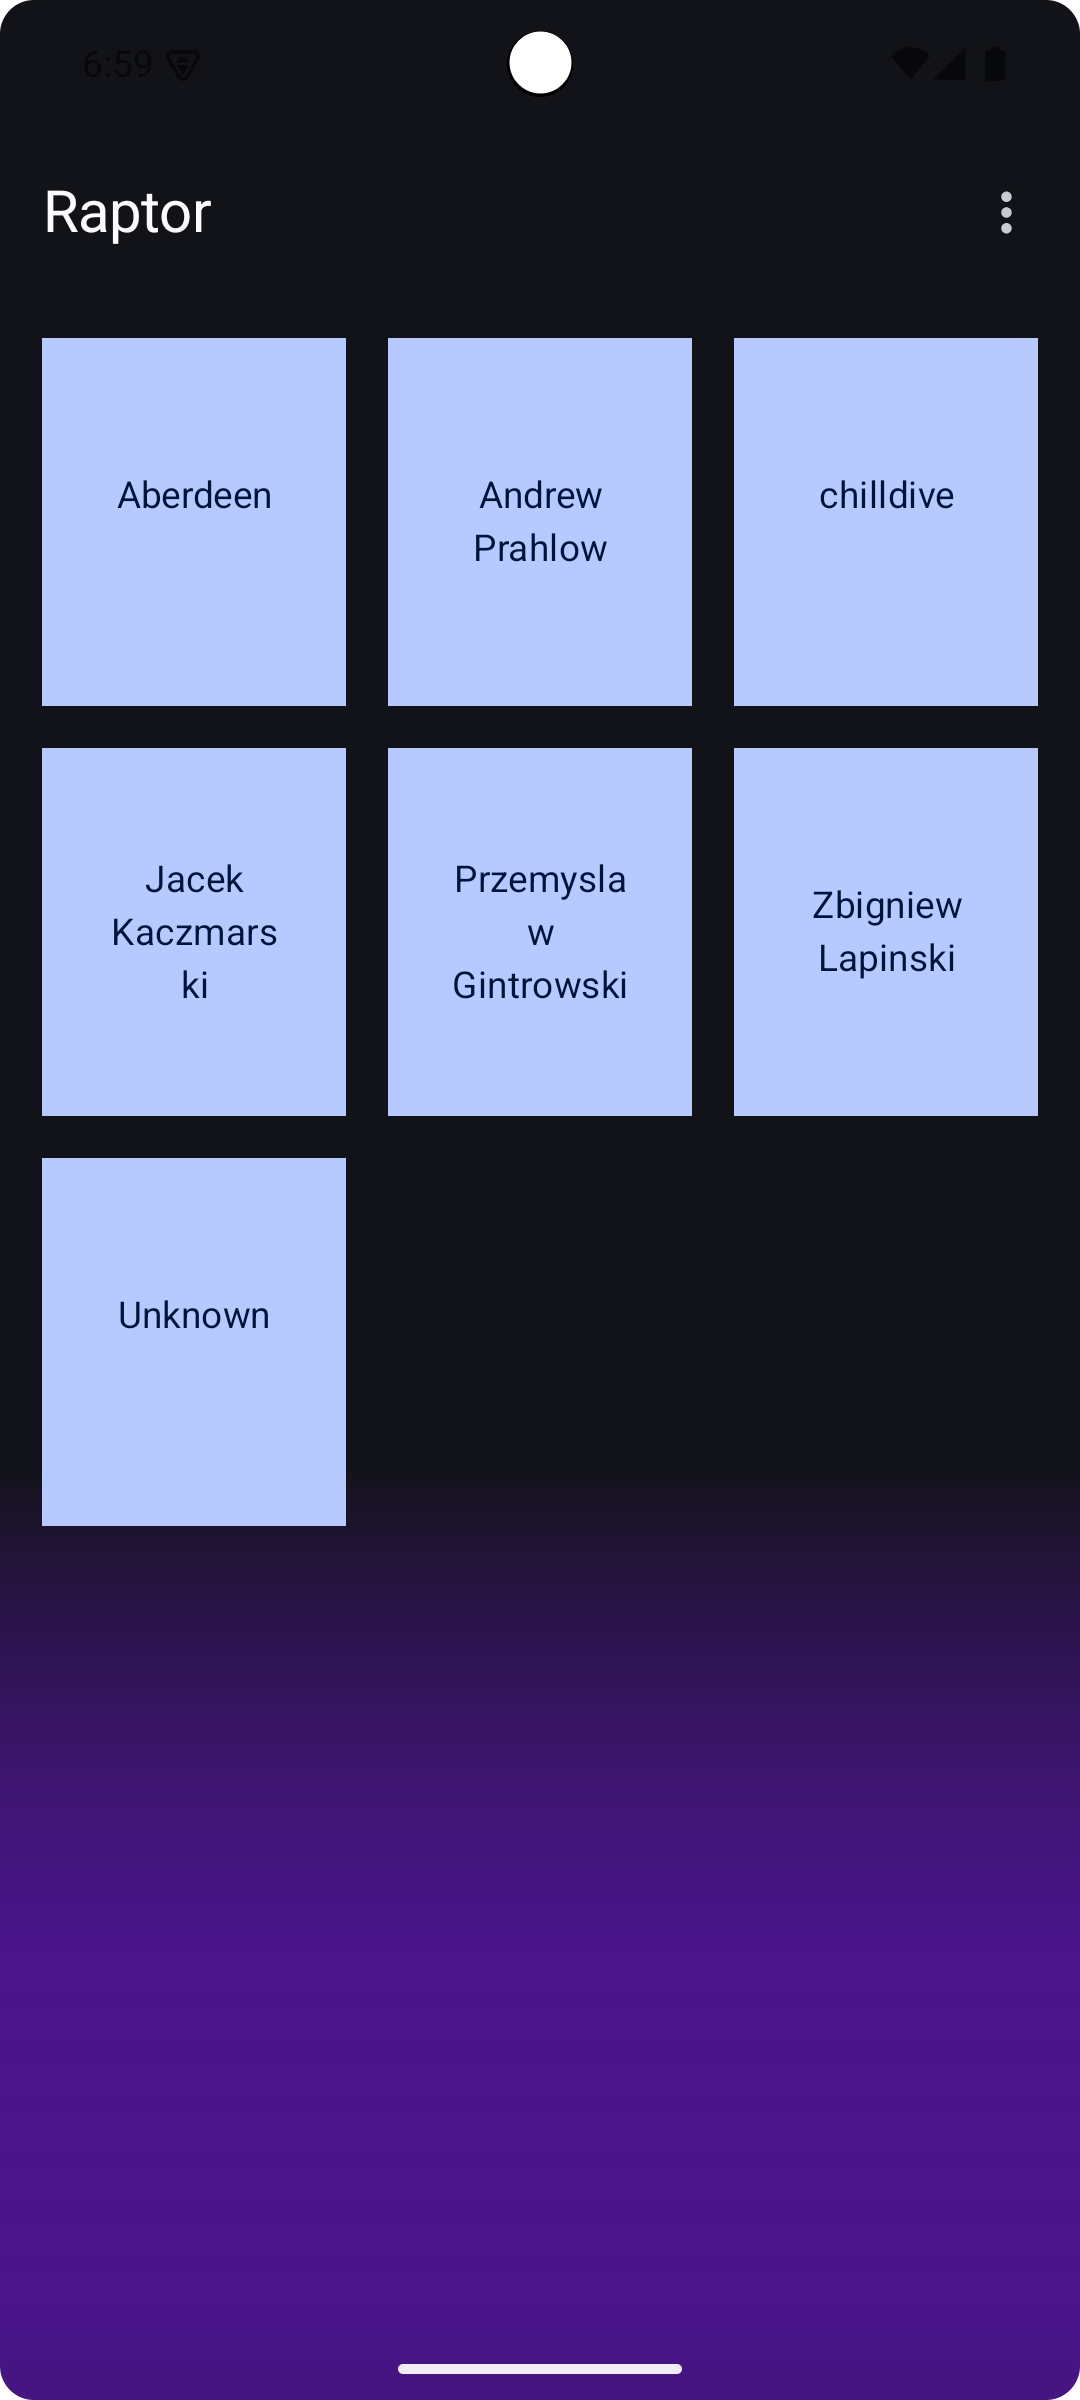
\includegraphics[width=1\textwidth]{images/tutorial_after_loading.png}
	\caption{\centering{Widok po załadowaniu plików.}}
	\label{fig:tutorial_after_loading}
\end{figure}

Użytkownik może teraz wejść w katalog albumów dowolnego autora, klikając na kafelek z jego nazwą. Przeniesie to użytkownika do widoku albumów, wyglądający jak na rysunku nr.~\ref{fig:tutorial_album_view}.

\begin{figure}[H]
	\centering
	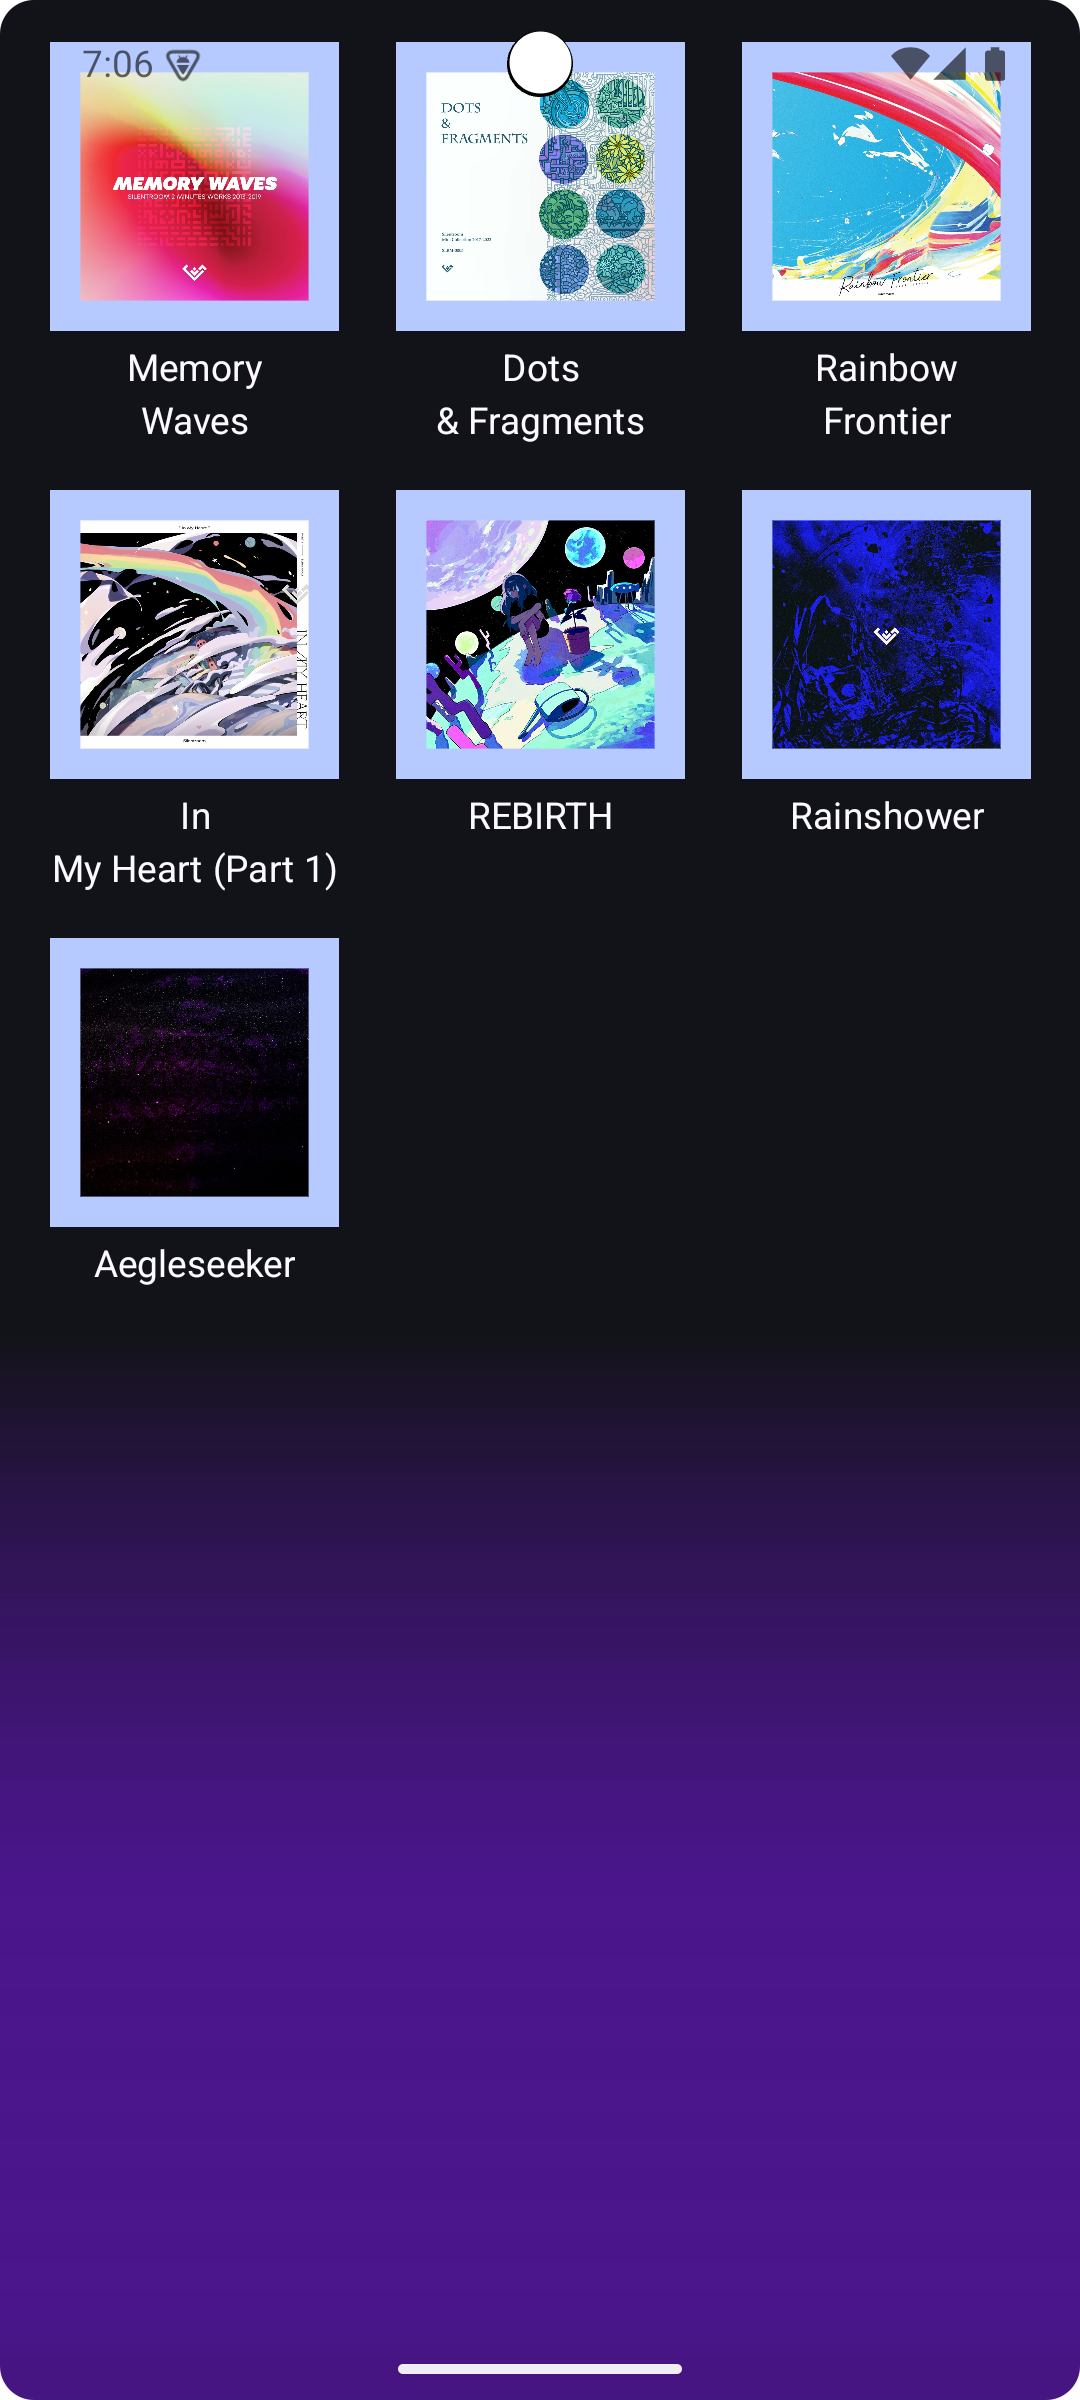
\includegraphics[width=1\textwidth]{images/tutorial_album_view.png}
	\caption{\centering{Widok po wejściu w autora.}}
	\label{fig:tutorial_album_view}
\end{figure}

Analogicznie, należy kliknąć na kafelek korespondujący do odpowiedniego albumu. Aplikacja wtedy przejdzie do widoku piosenek, gdzie można faktycznie wybrać piosenkę do odtworzenia, co pokazana no rys. nr.~\ref{fig:tutorial_song_view}. 

\begin{figure}[H]
	\centering
	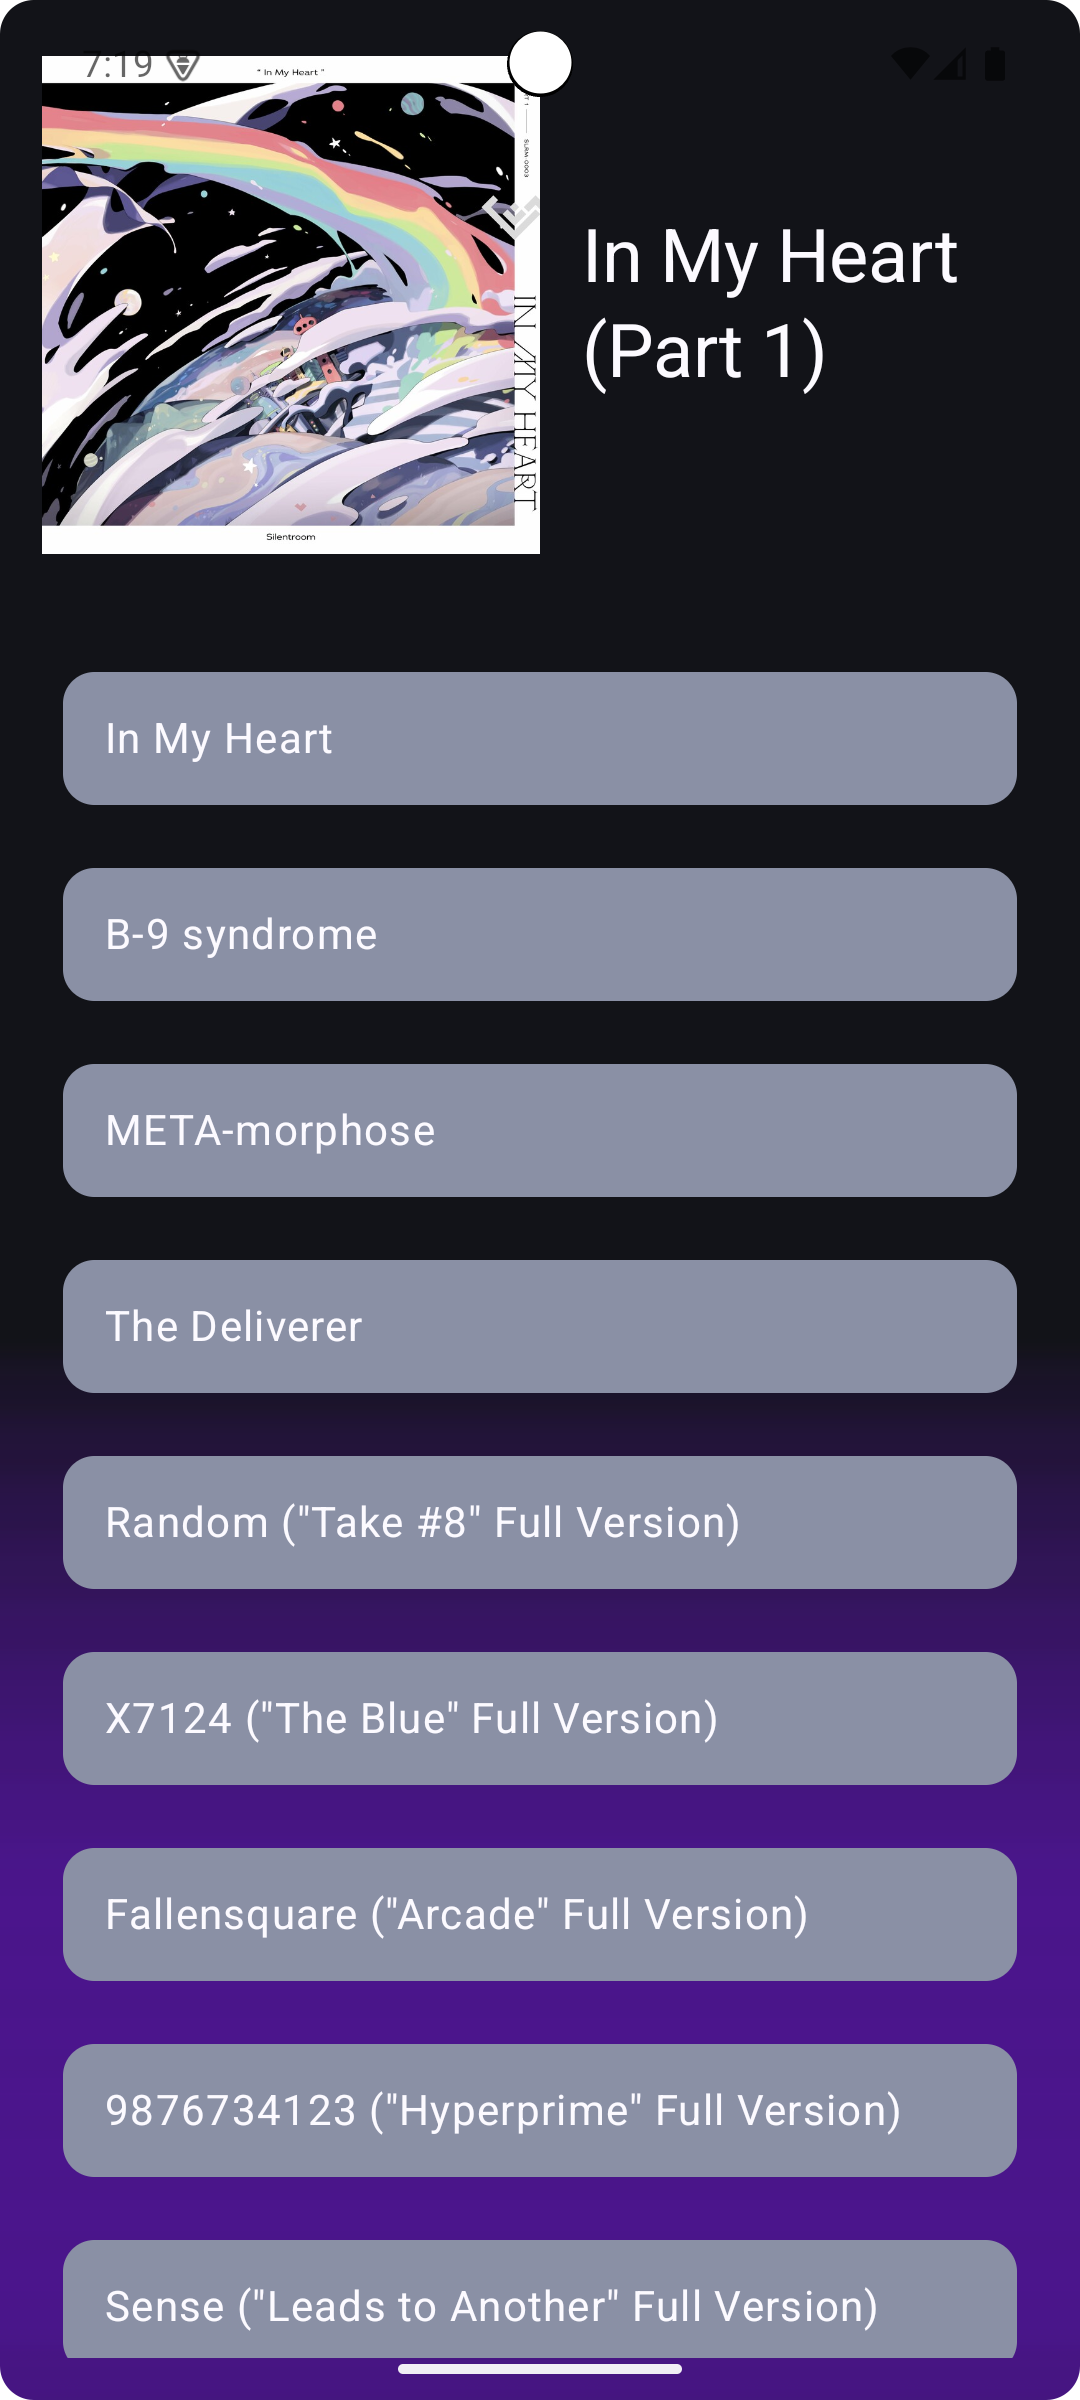
\includegraphics[width=1\textwidth]{images/tutorial_song_view.png}
	\caption{\centering{Widok wyboru piosenki.}}
	\label{fig:tutorial_song_view}
\end{figure}

Po wybraniu piosenki, aplikacja otwiera ekran odtwarzacza, pokazany na rys. nr.~\ref{fig:tutorial_player_view}

\begin{figure}[H]
	\centering
	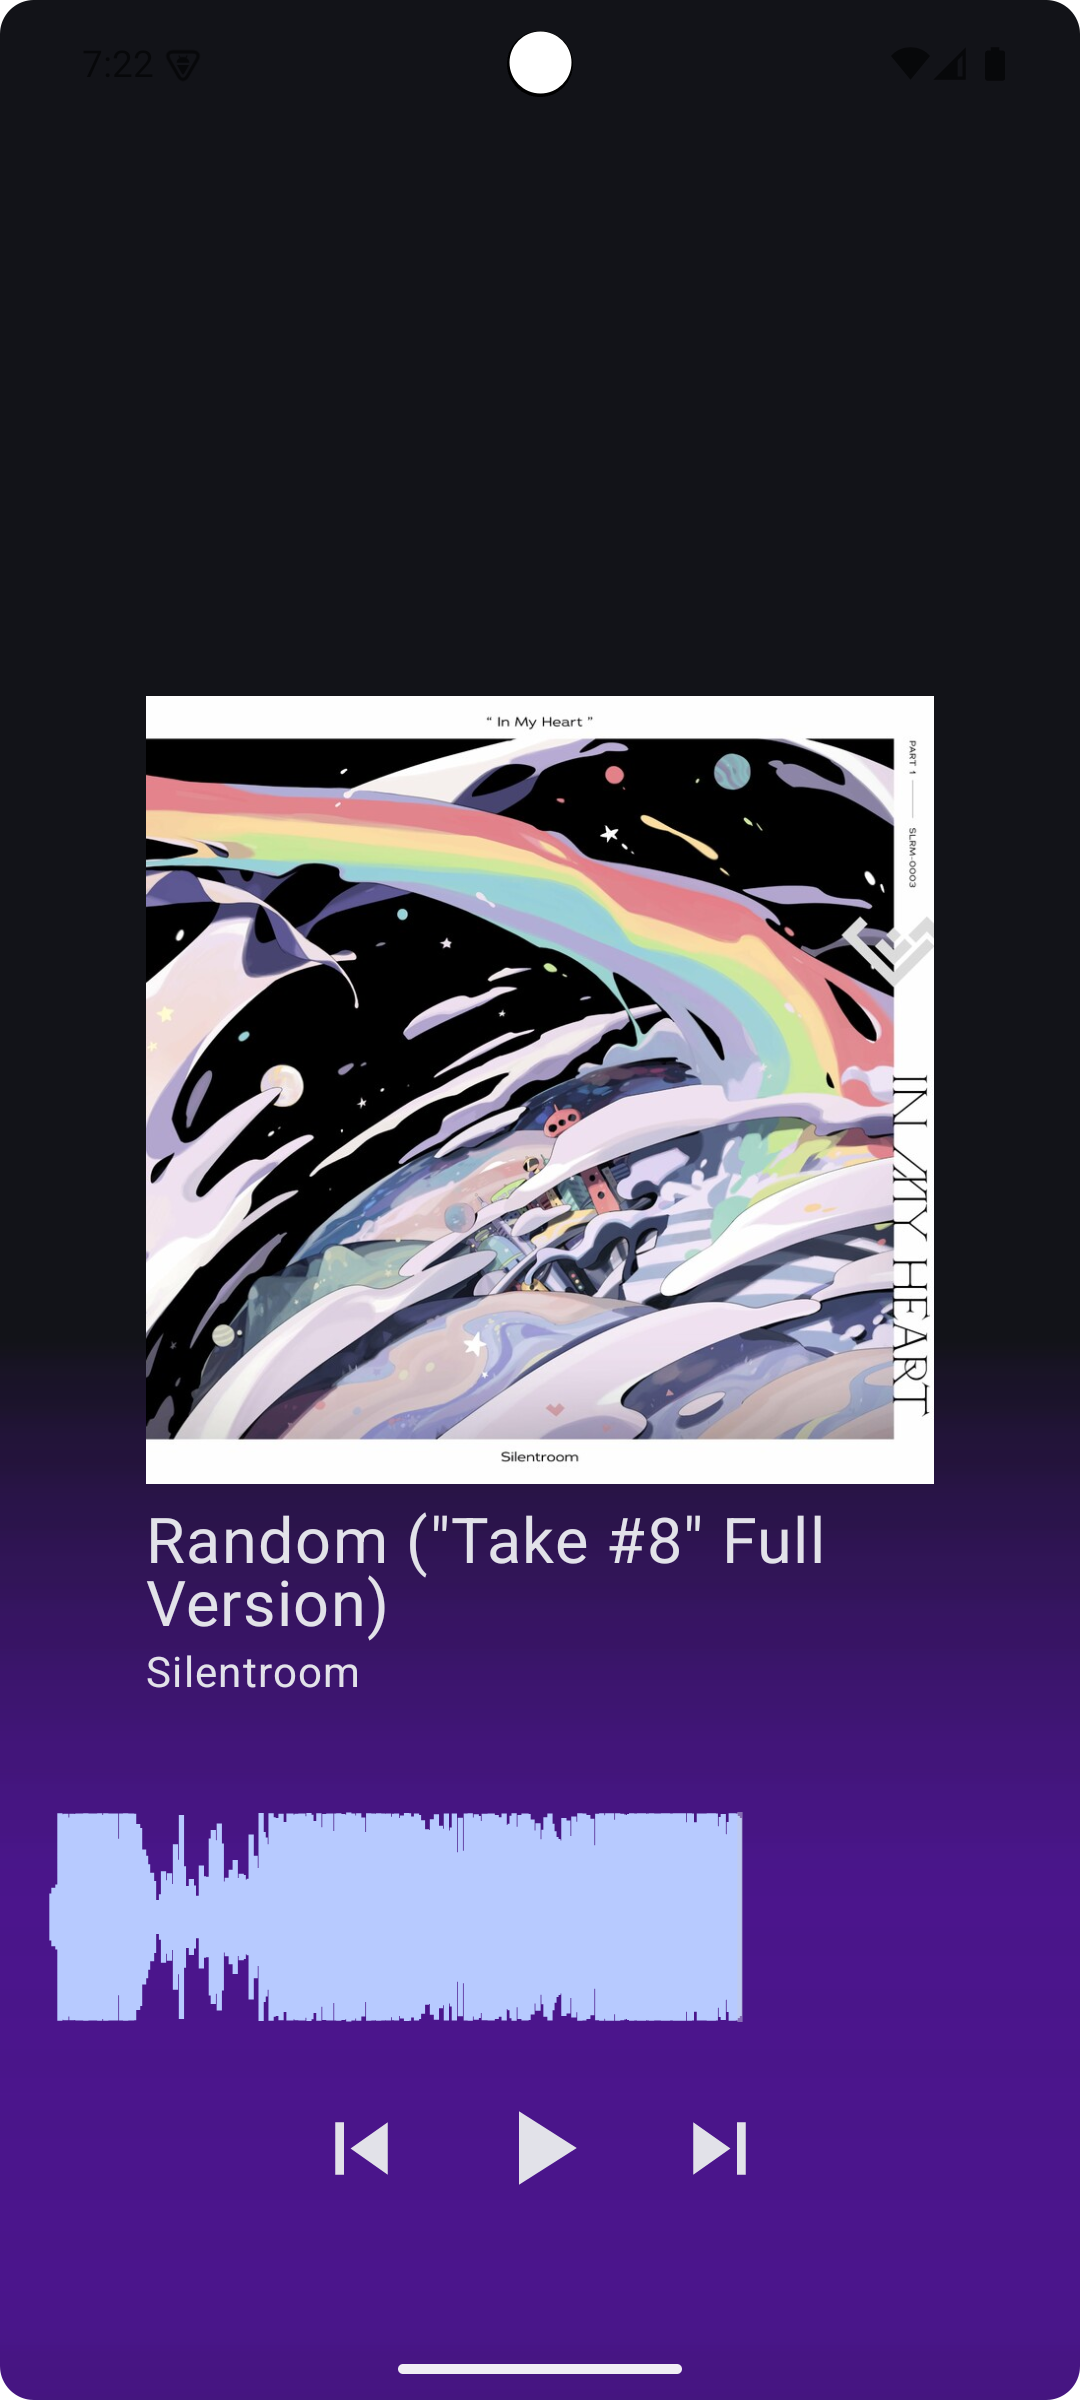
\includegraphics[width=1\textwidth]{images/tutorial_player_view.png}
	\caption{\centering{Widok odtwarzacza.}}
	\label{fig:tutorial_player_view}
\end{figure}

Waveform na dole odtwarzacza pokazuje postęp odtwarzania. Przycisk na środku, pod nim pełni funkcje odtwarzania, pauzowania i restartowania piosenki, zależnie od tego w jakim stanie jest odtwarzanie. Przyciski po lewej i prawej jego stronie odtwarzają poprzednie i następne utwory. Kolejność odtwarzania determinowana jest poprzez numer w albumie piosenki, jeżeli jest on w tagach. Czyli, dla piosenki o numerze 5, klikając w lewy przycisk, odtwarzanie przejdzie do piosenki o numerze 4 w albumie. Przy prawej strzałce, odtwarzanie przejdzie do piosenki nr. 6. Jeżeli użytkownik spróbuje przejść do piosenki, której numer nie istnieje w albumie, to aplikacja powiadomi go o tym, co widać na rys. nr.~\ref{fig:tutorial_player_lastsong}.

\begin{figure}[H]
	\centering
	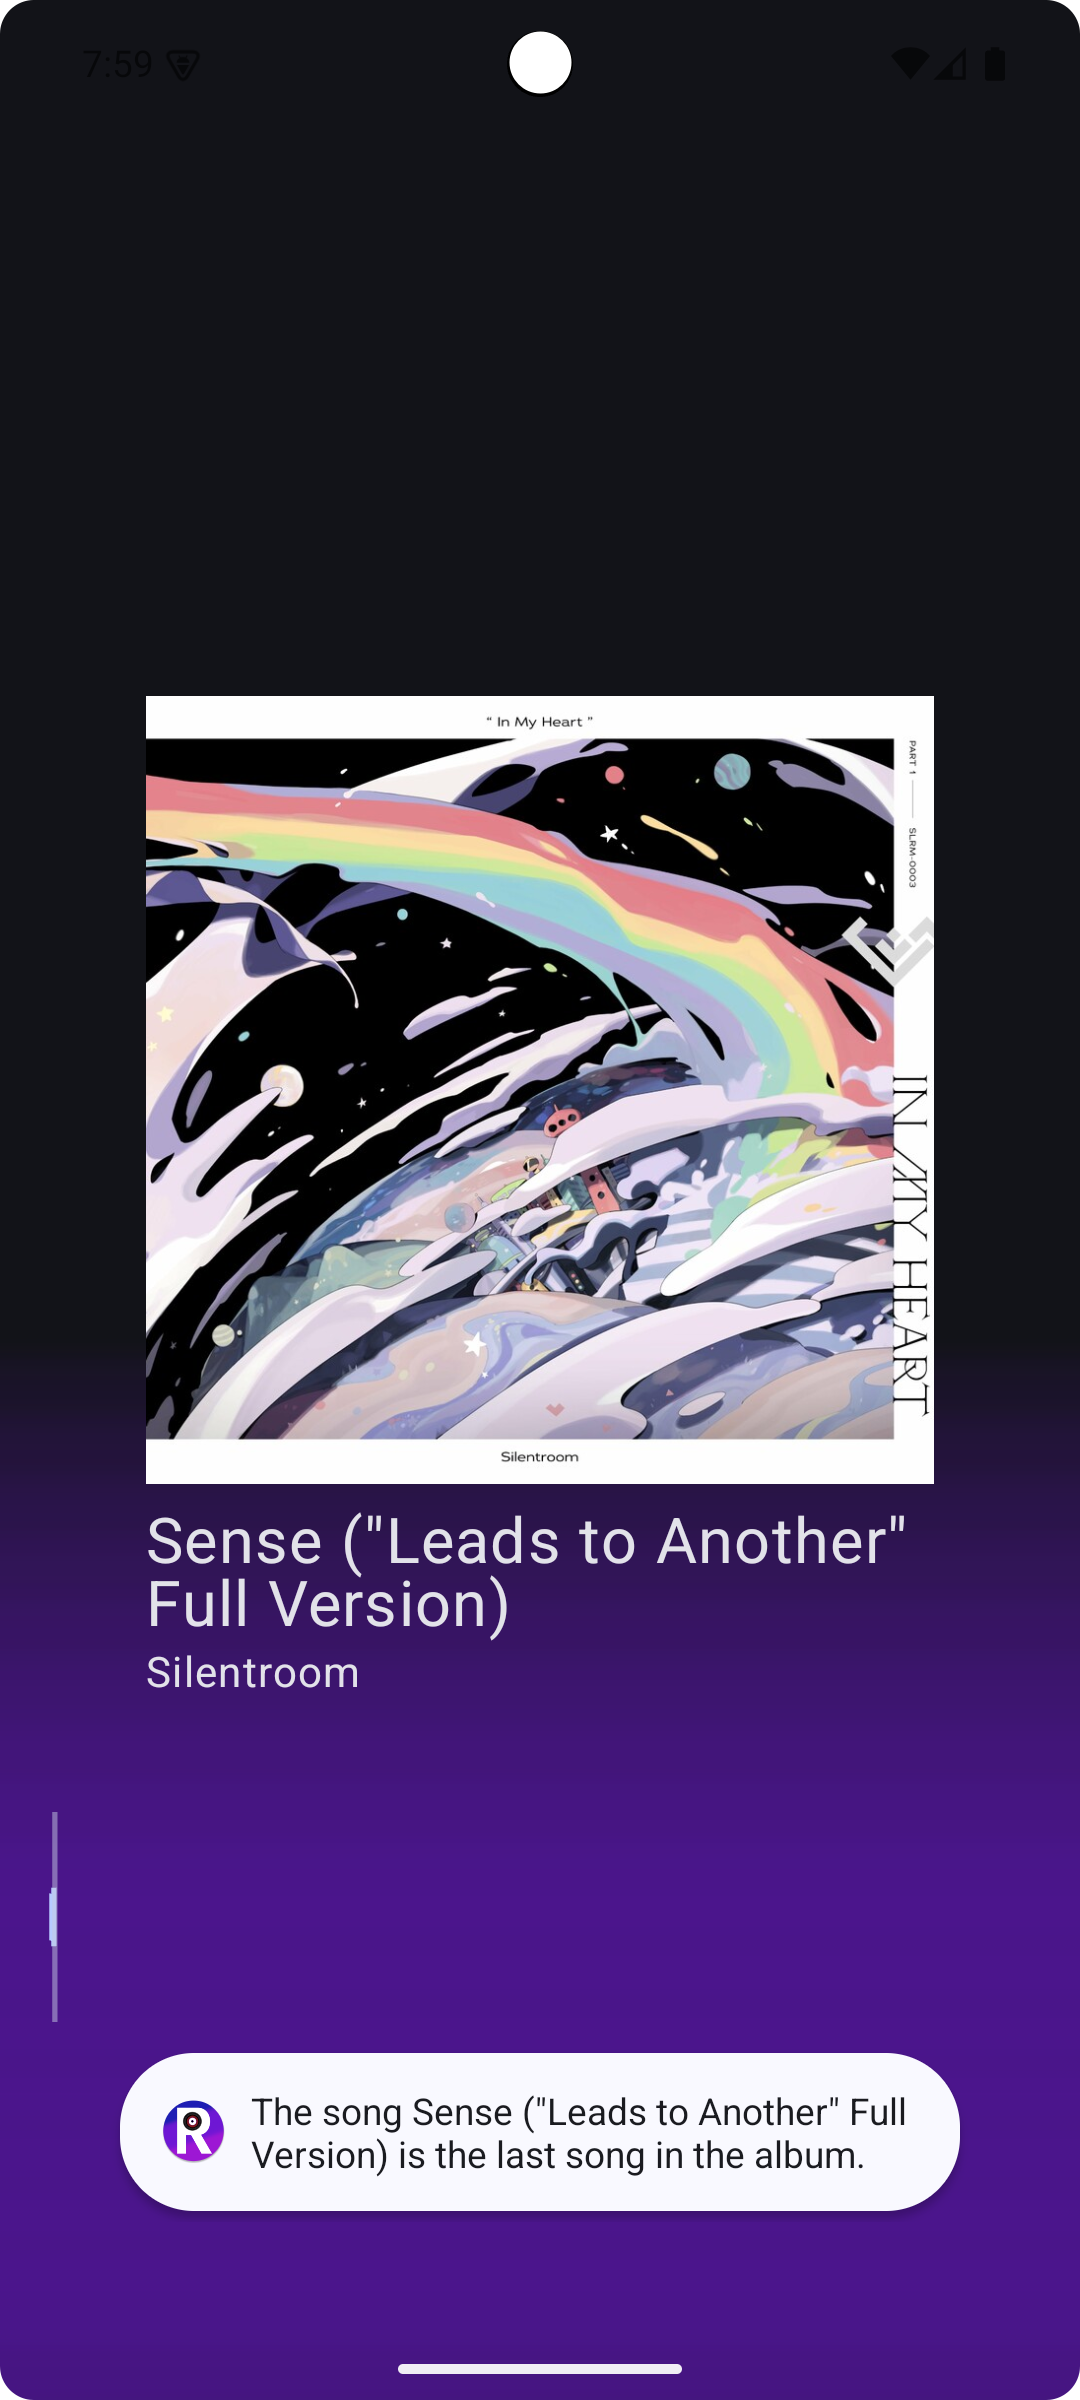
\includegraphics[width=1\textwidth]{images/tutorial_player_lastsong.png}
	\caption{\centering{Próba zagrania następnej piosenki, grając ostatnią.}}
	\label{fig:tutorial_player_lastsong}
\end{figure}

Można też zwrócić uwagę na inne funkcje aplikacji. Aplikacja obsługuje standardową nawigację w Androidzie, można wyjść z odtwarzacza wbudowanym przyciskiem w tył / przesunięciem palca, łącznie z innymi ekranami. Ponadto zademonstrować można inne czujniki obsługiwane przez aplikację. Jeżeli zwiększy się ilość światła, to aplikacja przejdzie w jasny tryb (bądź ciemny jeżeli światło się zmniejszy), jak pokazano na rys. nr.~\ref{fig:tutorial_light_sensor}.

\begin{figure}[H]
	\centering
	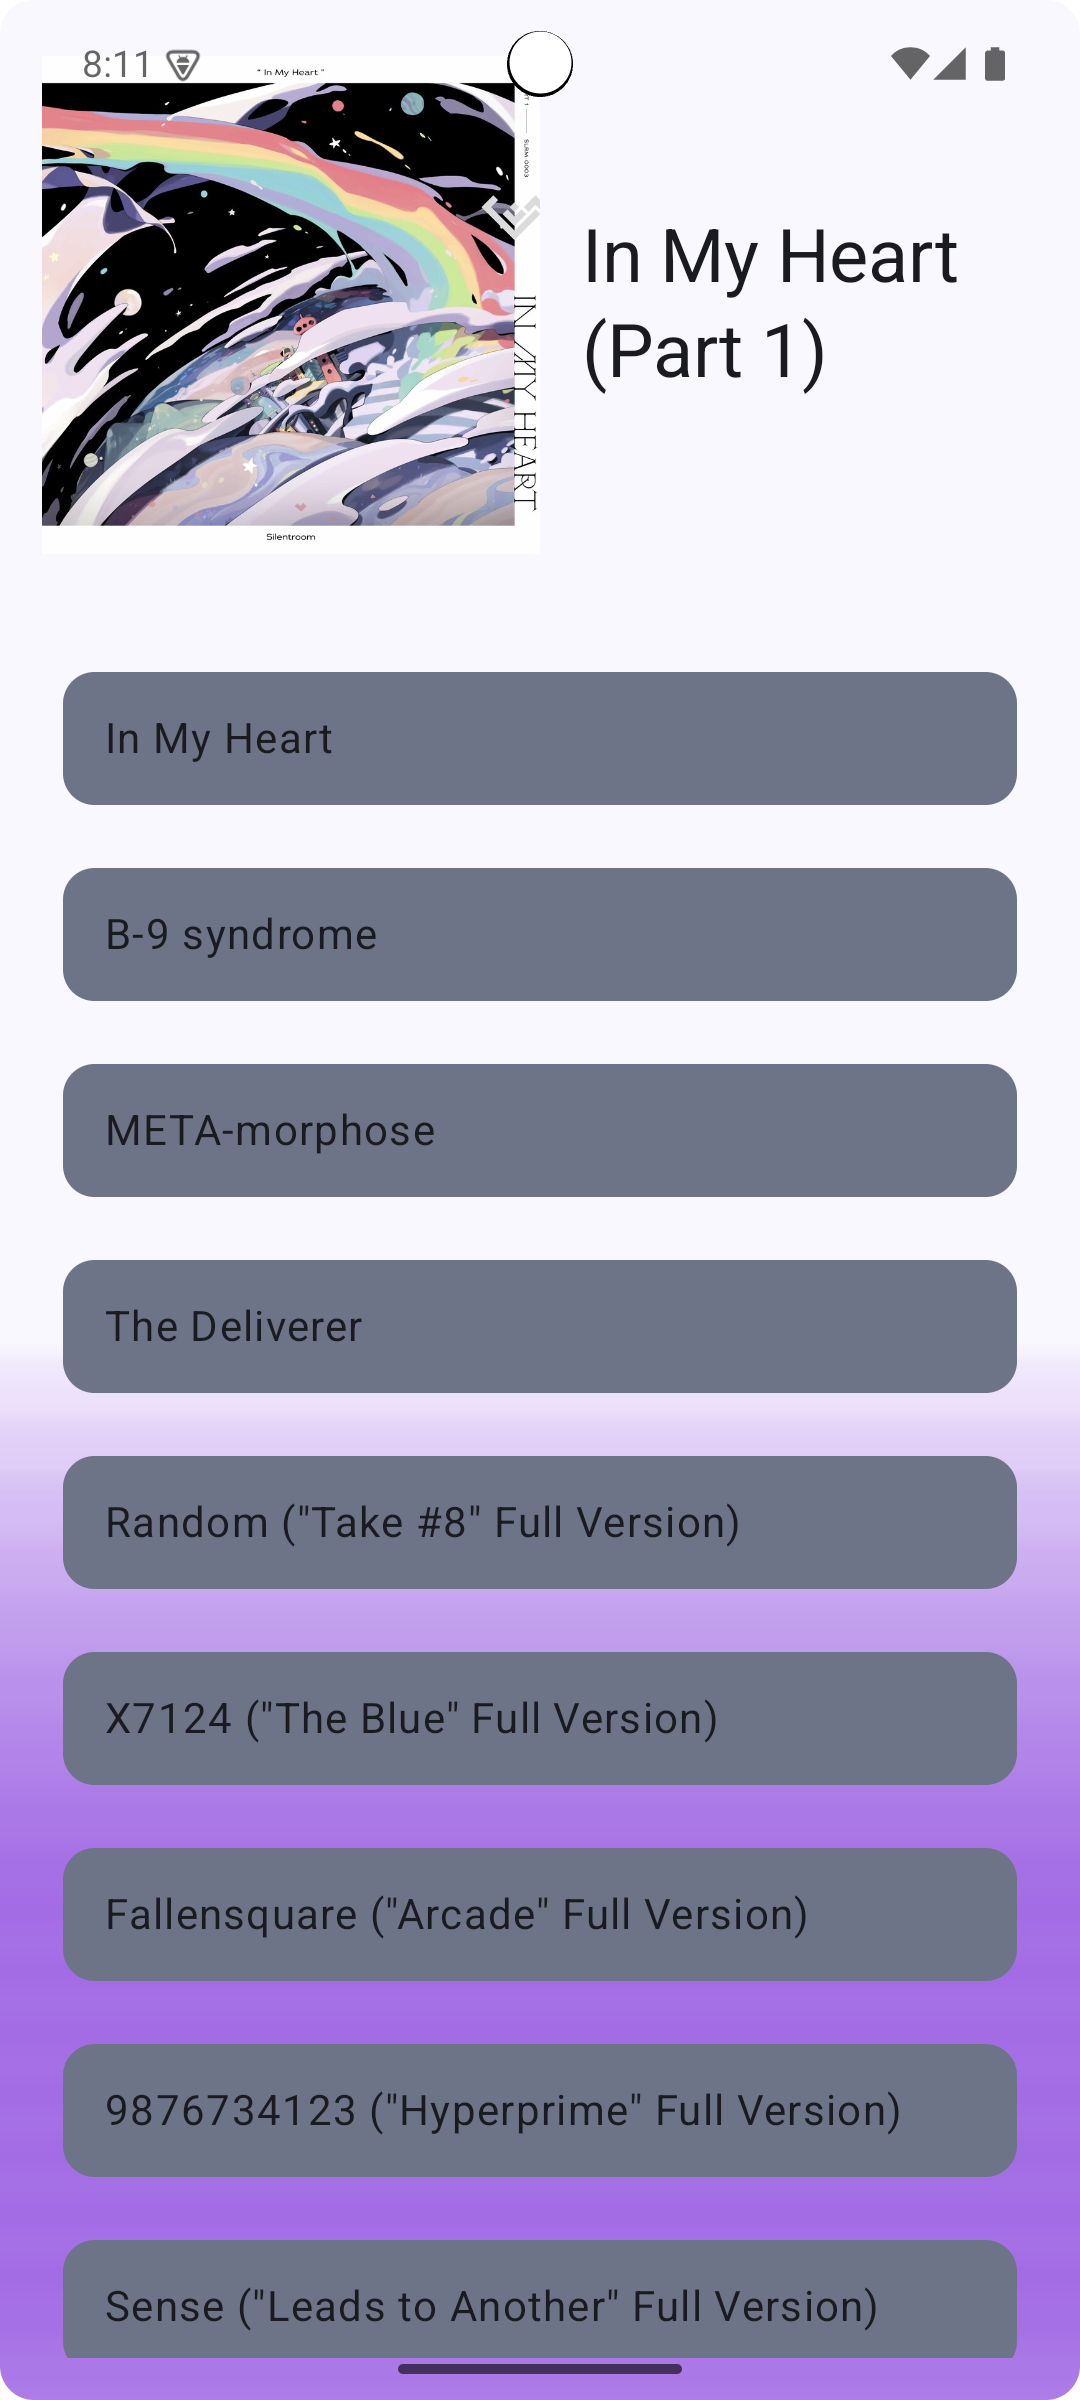
\includegraphics[width=1\textwidth]{images/tutorial_light_sensor.png}
	\caption{\centering{Aplikacja zmieniła kolorystykę na jasną.}}
	\label{fig:tutorial_light_sensor}
\end{figure}

Ekran można też obrócić o 90\degree, co zmieni nieco układ aplikacji. Pokazano to na rys. nr.~\ref{fig:tutorial_rotate}

\begin{figure}[H]
	\centering
	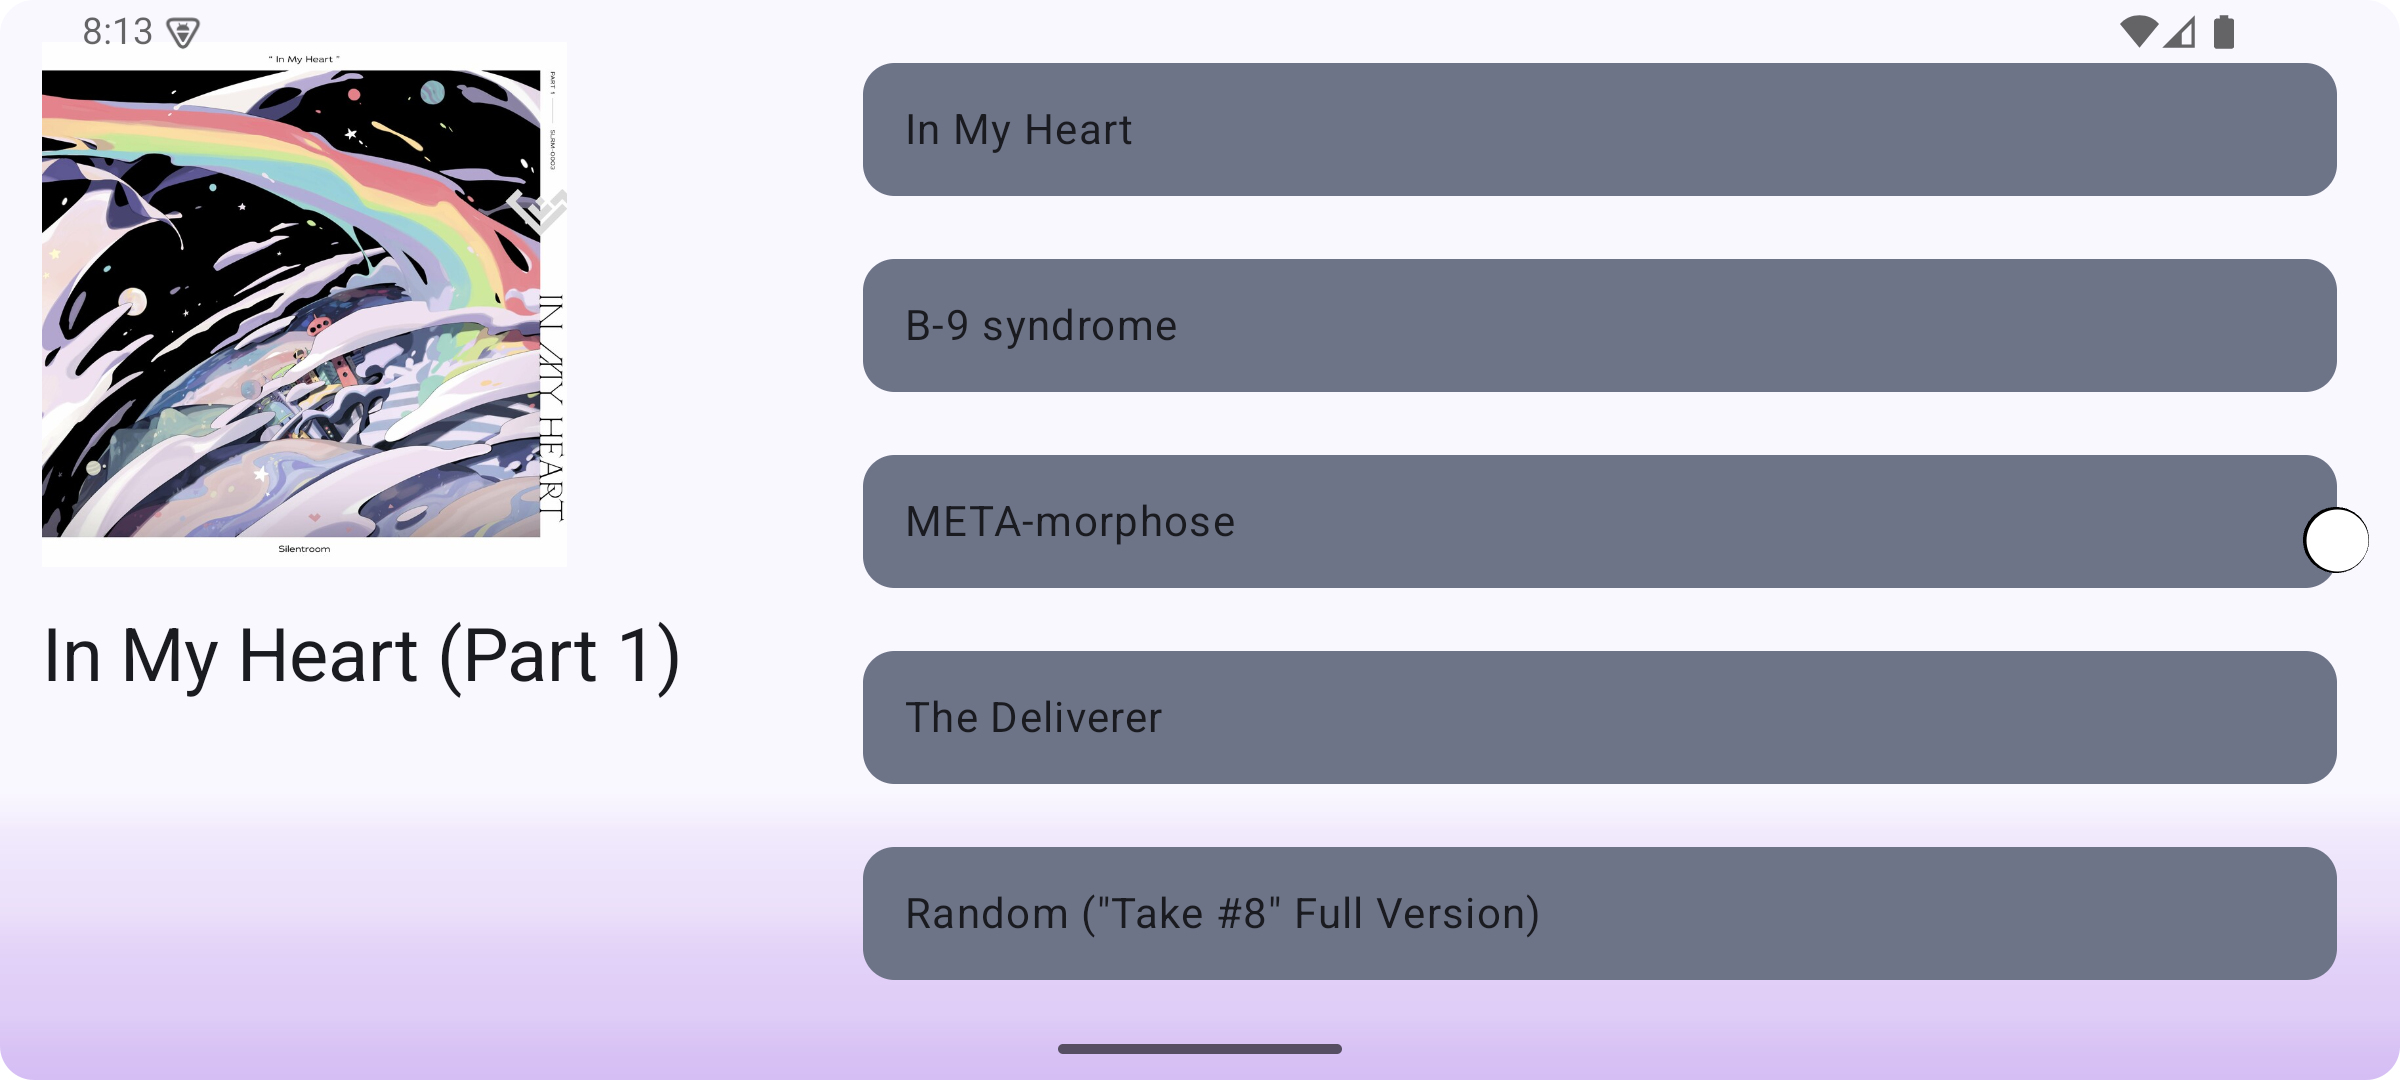
\includegraphics[width=1\textwidth]{images/tutorial_rotate.png}
	\caption{\centering{Obrócenie ekranu.}}
	\label{fig:tutorial_rotate}
\end{figure}
